In this chapter the experimental setup of this paper and the the corresponding code will be described. Referring to the chapter before, there are three different test that need to be conducted. 

\textbf{Setup Website} \newline
In order to do all tests in one place, a locally hosted website was created. The setup of this website is rather simple yet effective. It consists of a headline and six buttons.
\begin{figure}[H]
    \centering
    \caption[]{This is our website}
	\label{fig:website}
    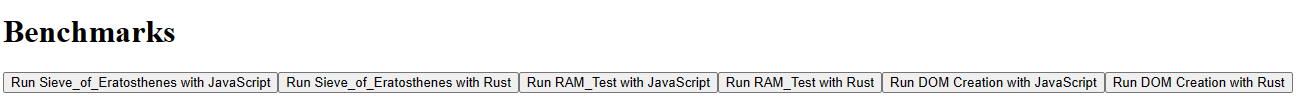
\includegraphics[width=1\textwidth]{website}
\end{figure}

Each button executes one of the tests, three buttons are for the JavaScript tests and the other three for the WASM tests. Before each test is executed, an input window appears and asks the user to enter a number. What the number represents depends on the test that is executed.

The code of the main page of the website looks as follows:
\begin{verbatim}
<!DOCTYPE html>
<html lang="en">
    <head>
        <meta charset="UTF-8">
        <meta name="viewport" content="width=device-width, initial-scale=1.0">
        <title>Benchmarks</title>
    </head>
    <body>
        <h1>Benchmarks</h1>
        <script type="module" src="./main.js"></script>
    </body>
</html>
\end{verbatim}
input caption here

This basic HTML Code defines the main structure of the website. In terms of styling, there is none. The main task of this code is to link the main.js file.  

\textbf{Setup First Test - CPU Benchmark} \newline
Next is the setup of the first test, which is a CPU Benchmark test based on the Sieve of Eratosthenes algorithm. In the field of computer science this algorithm is commonly used to measure computer performance. "The time complexity of calculating all primes below n in the random access machine model is \( O(n \log \log n) \) operations, a direct consequence of the fact that the prime harmonic series asymptotically approaches \( \log \log n\). It has an exponential time complexity with regard to input size, though, which makes it a pseudo-polynomial algorithm. The basic algorithm requires \( O(n) \) of memory." (!Quelle wikipedia Sieve of Eratosthenes).
The input parameter for this test determines the limit up to where the algorithm searches for prime numbers.

The following code was used to execute the algorithm with JavaScript:
\begin{verbatim}
function js_sieve(limit) {
    // Create an array to track whether each number is prime
    const sieve = new Array(Number(limit) + 1).fill(true);
    // 0 and 1 are not prime numbers, so mark them as false
    sieve[0] = sieve[1] = false;
    // Initialize an empty array to store prime numbers
    const primes = [];
    // Iterate through the numbers starting from 2 up to the square root of the limit
    for (let i = 2; i <= Math.sqrt(limit); i++) {
        // If the current number is prime (marked as true), proceed
        if (sieve[i]) {
            // Mark multiples of the current prime number as not prime
            // Starting from i*i, as all numbers below that would have been already marked
            for (let j = i ** 2; j <= limit; j += i) {
                sieve[j] = false;
            }
        }
    }
    // Iterate through the sieve to extract prime numbers
    for (let i = 0; i < sieve.length; i++) {
        if (sieve[i]) {
            primes.push(i);
        }
    }
    // Return the array of prime numbers
    return primes;
}
\end{verbatim}
caption einfügen

The following code was used to execute the algorithm with WASM, coded in Rust:
\begin{verbatim}
#[wasm_bindgen]
pub fn wasm_sieve(limit: usize) -> Vec<usize> {
    // Create a boolean vector to track whether each number is prime
    let mut sieve: Vec<bool> = vec![true; limit + 1];
    let mut primes: Vec<usize> = Vec::new();
    // 0 and 1 are not prime numbers, so mark them as false
    sieve[0] = false;
    sieve[1] = false;
    // Iterate through the numbers starting from 2 up to the square root of the limit
    for i in 2..=(limit as f64).sqrt() as usize {
        // If the current number is prime (marked as true), proceed
        if sieve[i] {
            // Mark multiples of the current prime number as not prime
            // Starting from i*i, as all numbers below that would have been already marked
            for j in (i * i..=limit).step_by(i) {
                sieve[j] = false;
            }
        }
    }
    // Iterate through the sieve to extract prime numbers
    for i in 2..=limit {
        if sieve[i] {
            primes.push(i);
        }
    }
    // Return the vector of prime numbers
    primes
}
\end{verbatim}
caption einfügen 

Both code snippets in essence implement the same algorithm, just in different languages. However, it was coded in such a way that the implementations are comparable. To give an example, the code written in Rust could be further optimized by iterating over the sieve vector with `sieve.iter()`. Since this is not an option in JavaScript it was implemented similarly to JavaScript to enhance comparability. Another difference between both implementations is the usage of vectors in Rust. Because the neither the input nor the number of primes is not known beforehand, a growable object is required. In JavaScript an array is such a growable object but in Rust an array is not growable, therefore it is replaced by a vector. 

\textbf{Setup Second Test - RAM Speed} \newline
The second test uses a multitude of read and write operations as a stress test for the RAM speed. The input parameter for this test determines the size of the iterable to perform the read and write operations on.

The following code was used to execute the algorithm with JavaScript:
\begin{verbatim}
function js_ram_test(size) {
    const array = new Array(size);
    // Write operation
    for (let i = 0; i < size; i++) {
        array[i] = i;
    }
    // Read operation
    for (let i = 0; i < size; i++) {
        array[i] += 1;
    }
}
\end{verbatim}
caption einfügen

The following code was used to execute the algorithm with WASM, coded in Rust:
\begin{verbatim}
#[wasm_bindgen]
pub fn wasm_ram_test(size: usize) {
    let mut vec: Vec<usize>  = Vec::with_capacity(size);
    // Write operation
    for i in 0..size {
        vec.push(i);
    }
    // Read operation
    for i in 0..size {
        vec[i] += 1;
    }
}
\end{verbatim}
caption einfügen

As with the first test, the two code snippets, in essence, execute the same operations. The difference in both implementations are identical to the previous test and are also justified the same way. 

\textbf{Setup Second Test - DOM manipulation} \newline
The final test was about DOM manipulation and was implemented because JavaScript "makes it relatively easy to manipulate the DOM (i.e., add, modify, and remove elements), but does nothing to promote doing so efficiently" (!Quelle toptal The 10 Most Common JavaScript Issues Developers Face). Therefore this test investigates the DOM manipulation with JavaScript and WASM to see which operates more efficiently. The input parameter for this test determines the number of div elements that should be created and shown on the screen.

The following code was used to execute the algorithm with JavaScript:
\begin{verbatim}
function js_create_elements(count) {
    // Get a reference to the document body
    const body = document.body;
    // Iterate 'count' times to create elements
    for (let i = 0; i < count; i++) {
        // Create a new div element
        const div = document.createElement("div");
        // Set styles for the div element
        div.style.border = "2px solid #000";
        div.style.backgroundColor = "#e0e0e0";
        div.style.margin = "5px";
        // Set text content for the div element
        div.textContent = "Hello, JavaScript!";
        // Append the div element to the document body
        body.appendChild(div);
    }
}
\end{verbatim}
caption einfügen

The following code was used to execute the algorithm with WASM, coded in Rust:
\begin{verbatim}
#[wasm_bindgen]
pub fn wasm_create_elements(count: usize) {
    // Access the document object from the web_sys crate
    let document = web_sys::window().unwrap().document().unwrap();
    // Iterate 'count' times to create elements
    for _ in 0..count {
        // Create a new div element
        let div = document.create_element("div").unwrap();
        // Set styles for the div element
        div.set_attribute("style", "border: 2px solid #000; background-color: #e0e0e0; margin: 5px;").unwrap();
        // Set text content for the div element
        div.set_text_content(Some("Hello, WASM!"));
        // Append the div element to the document body
        document.body().unwrap().append_child(&div).unwrap();
    }
}
\end{verbatim}
caption einfügen

In this case the two code snippet again implement the same procedure. Unlike in the previous tests, there are no performance-relevant differences between JavaScript and WASM. The difference in the code emerge from the syntax of the two languages. However, one difference needs to be highlighted. Rust encourages explicit error handling. Since this code will not be deployed to regular users, explicit error handling is not necessary and is avoided by using the `.unwrap()` function.

One aspect of all Rust-specific tests is the \texttt{\#[wasm\_bindgen]} command before every function which is described by mdn web docks as follows "wasm-pack uses wasm-bindgen, another tool, to provide a bridge between the types of JavaScript and Rust. It allows JavaScript to call a Rust API with a string, or a Rust function to catch a JavaScript exception" (!Quelle? mozilla compiling from rust to WASM). This command is essential for the main.js to access the Rust functions when a test is triggered, therefore it is another important of this chapter. 